\documentclass[]{article}
\usepackage[brazil]{babel}
\usepackage{graphicx}
\usepackage{mathtools}
\usepackage{float} 
\usepackage{xcolor}
\usepackage{amsmath, amssymb, bm}


\usepackage{array}
\usepackage{booktabs}



% margenes
\usepackage[a4paper,left=3cm,right=3cm,top=3cm]{geometry}

%opening
\title{}
\author{}

\begin{document}

\begin{center}
	{\tiny {\normalsize {\large Lista de exercicios 1\\
Convecçao\\
\textbf{Cristian Herledy Lopez Lara}}}}
\end{center}

\section*{Exercício 1}
\subsubsection*{1.1}

\textbf{Derivar, a partir de um volume infinitesimal, as equações da conservação da massa, momento e energia na forma diferencial.} \\


\textbf{Conservação da massa:} 

Considerando um volume de controle fixo dentro do campo de fluxo (com $\Delta x \Delta y  \Delta z \rightarrow 0 $), infinitesimalmente pequeno, a abordagem para conservação de massa será:

\begin{equation}
	\frac{\Delta m}{\Delta t} = \dot{m}_{entra} - \dot{m}_{sai}
\end{equation}
OBSERVAÇÃO: Para facilidade, os diagramas de equilíbrio são desenhados em duas dimensões.

\begin{figure}[H]
	\centering
	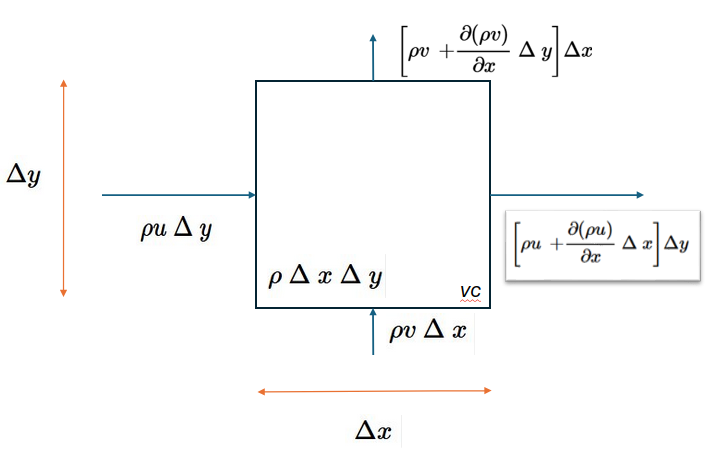
\includegraphics[width=.65\textwidth]{Figures/1_1.png}
	\caption{Conservação de massa em volume infinitesimal}
\end{figure}


Sua forma diferencial seria dada por

\begin{equation}
	\begin{aligned}
		\frac{\partial}{\partial t} (\rho \Delta x \Delta y \Delta z) = \rho u\Delta y\Delta z + \rho v\Delta x\Delta z + \rho w\Delta y\Delta z - [\rho u +	\frac{\partial}{\partial x}(\rho u)\Delta x]\Delta y\Delta z - \\ [\rho v +	\frac{\partial}{\partial y}(\rho v)\Delta y]\Delta x\Delta z - [\rho w +	\frac{\partial}{\partial z}(\rho w)\Delta z]\Delta x\Delta y
	\end{aligned}
\end{equation}

E dividindo pelo volume constante $\Delta x \Delta y  \Delta z$

\begin{equation}
	\begin{aligned}
		\frac{\partial}{\partial t} \rho + \frac{\partial}{\partial t} (\rho u) + \frac{\partial}{\partial t} (\rho v) + \frac{\partial}{\partial t} (\rho z) = 0 
	\end{aligned}
\end{equation}

Usando a definição de derivada material e o operador divergencia
\begin{equation}
	\begin{aligned}
		\frac{D}{D t} \rho +  \bigtriangledown (\rho V)= 0 
	\end{aligned}
\end{equation}


\textbf{Conservação do momento:} 

Derivando a análise da segunda lei de Newton e tomando a velocidade como uma propriedade de transporte, o abordagem para conservação do momento dentro do volume de controle (vc) será

\begin{equation}
	\frac{\Delta }{\Delta t} (mV)_{vc}= \sum F +\dot{m}V_{entra} - \dot{m}V_{sai}
\end{equation}

\begin{figure}[H]
	\centering
	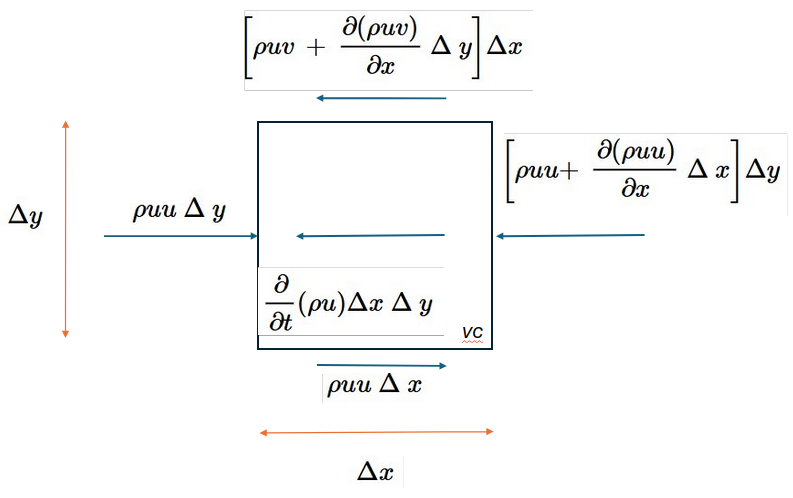
\includegraphics[width=.65\textwidth]{Figures/1_2}
	\caption{Balanço de forças devido ao fluxo de momento em volume infinitesimal}
\end{figure}

\begin{figure}[H]
	\centering
	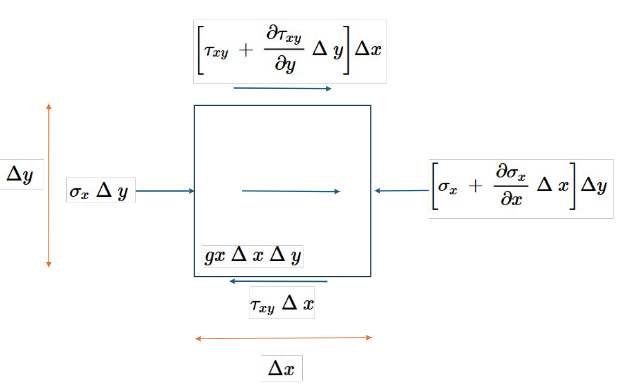
\includegraphics[width=.65\textwidth]{Figures/1_3}
	\caption{Balanço de forças devido a esforços normal e tangencial, e pelos terminos fonte}
\end{figure}

O equilíbrio de forças devido ao fluxo de momento e à tensão normal e tangencial na direção x será

\begin{equation}
	\begin{aligned}
		-\frac{\partial}{\partial t} (\rho u \Delta x \Delta y \Delta z) + \rho uu \Delta y \Delta z - [\rho uu +	\frac{\partial}{\partial x}(\rho uu)\Delta x]\Delta y\Delta z - \\  \rho uv \Delta x \Delta z - [\rho uv +	\frac{\partial}{\partial y}(\rho uv)\Delta y]\Delta x\Delta z -   \rho uw \Delta x \Delta y - [\rho uw +	\frac{\partial}{\partial z}(\rho uw)\Delta z]\Delta x\Delta y \\ + \sigma_{x} \Delta x\Delta y - (\sigma_{x} + \frac{\partial}{\partial x}\sigma_{x} \Delta x) \Delta y\Delta z - \tau_{xy} \Delta x\Delta y - (\tau_{xy} + \frac{\partial}{\partial x}\tau_{xy} \Delta y) \Delta x\Delta z + gx \Delta x\Delta y\Delta z
	\end{aligned}
\end{equation}

Sendo $gx$ o termo fonte. Dividindo pelo volume de controle quando $\Delta x \Delta y  \Delta z \rightarrow 0 $

\begin{equation}
	\begin{aligned}
		\rho \frac{ Du}{Dt} + u[ \frac{D}{D t} \rho + \rho(\frac{\partial}{\partial x}u \frac{\partial}{\partial y}v)] = - \frac{\partial \sigma_{x}}{\partial x} +  \frac{\partial \tau_{xy}}{\partial y} + gx   
	\end{aligned}
\end{equation}

Lembrando que o segundo termo é igual a zero segundo a conservação da massa

\begin{equation}
	\begin{aligned}
		\rho \frac{ Du}{Dt} = - \frac{\partial \sigma_{x}}{\partial x} +  \frac{\partial \tau_{xy}}{\partial y} + gx   
	\end{aligned}
\end{equation}

Com a definição do tensor de tensão dada por
\begin{equation}
	\tau_{ij} = -p \delta_{ij} + \mu \left( \frac{\partial u_i}{\partial x_j} + \frac{\partial u_j}{\partial x_i} \right) + \delta_{ij} \lambda \nabla \cdot \mathbf{V}
\end{equation}
\begin{equation}
	\lambda = -\frac{2}{3} \mu
\end{equation}

Que combinado com a equação 8 dá origem à equação de Navier-Stokes em x
\begin{equation}
	\begin{aligned}
	\frac{\partial}{\partial t} (\rho u) + \frac{\partial}{\partial x} (\rho u u) + \frac{\partial}{\partial y} (\rho v u) + \frac{\partial}{\partial z} (\rho w u) = \\
	- \frac{\partial p}{\partial x} + \frac{\partial}{\partial x} \left( 2 \mu \frac{\partial u}{\partial x} + \lambda \nabla \cdot \mathbf{V} \right) +
	\frac{\partial}{\partial y} \left( \mu \left( \frac{\partial u}{\partial y} + \frac{\partial v}{\partial x} \right) \right) +
	\frac{\partial}{\partial z} \left( \mu \left( \frac{\partial u}{\partial z} + \frac{\partial w}{\partial x} \right) \right) + g_x
	\end{aligned}
\end{equation}

E para $y$ e $z$

\begin{equation}
	\begin{aligned}
	\frac{\partial}{\partial t} (\rho v) + \frac{\partial}{\partial x} (\rho u v) + \frac{\partial}{\partial y} (\rho v v) + \frac{\partial}{\partial z} (\rho w v) = \\
	- \frac{\partial p}{\partial y} + \frac{\partial}{\partial x} \left( \mu \left( \frac{\partial v}{\partial x} + \frac{\partial u}{\partial y} \right) \right) +
	\frac{\partial}{\partial y} \left( 2 \mu \frac{\partial v}{\partial y} + \lambda \nabla \cdot \mathbf{V} \right) +
	\frac{\partial}{\partial z} \left( \mu \left( \frac{\partial v}{\partial z} + \frac{\partial w}{\partial y} \right) \right) +  g_y
	\end{aligned}
\end{equation}

\begin{equation}
	\begin{aligned}
	\frac{\partial}{\partial t} (\rho w) + \frac{\partial}{\partial x} (\rho u w) + \frac{\partial}{\partial y} (\rho v w) + \frac{\partial}{\partial z} (\rho w w) = \\
	- \frac{\partial p}{\partial z} + \frac{\partial}{\partial x} \left( \mu \left( \frac{\partial w}{\partial x} + \frac{\partial u}{\partial z} \right) \right) +
	\frac{\partial}{\partial y} \left( \mu \left( \frac{\partial w}{\partial y} + \frac{\partial v}{\partial z} \right) \right) +
	\frac{\partial}{\partial z} \left( 2 \mu \frac{\partial w}{\partial z} + \lambda \nabla \cdot \mathbf{V} \right) +  g_z
	\end{aligned}
\end{equation}

\textbf{Conservação da energia:} 

Da mesma forma, o diagrama a seguir mostra a análise da primeira lei da termodinâmica para volume infinitesimal

\begin{figure}[H]
	\centering
	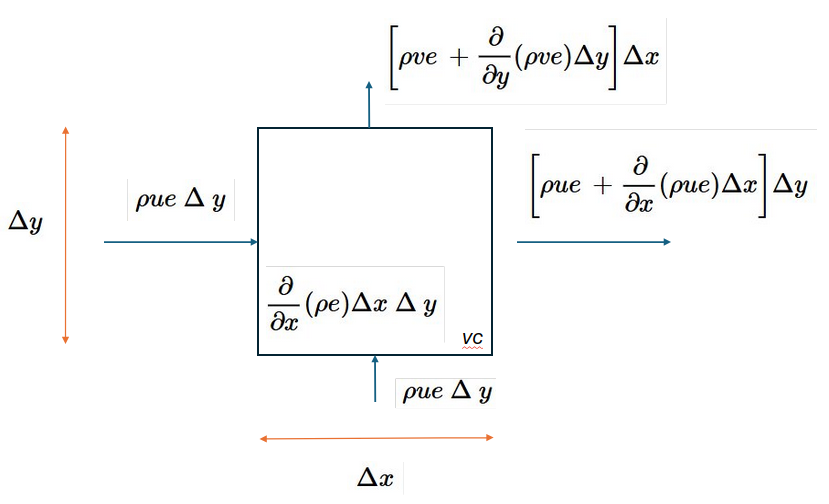
\includegraphics[width=.65\textwidth]{Figures/1_4}
	\caption{Equilíbrio da primeira lei da termodinâmica em volume infinitesimal pelo fluxo do fluido}
\end{figure}

\begin{figure}[H]
	\centering
	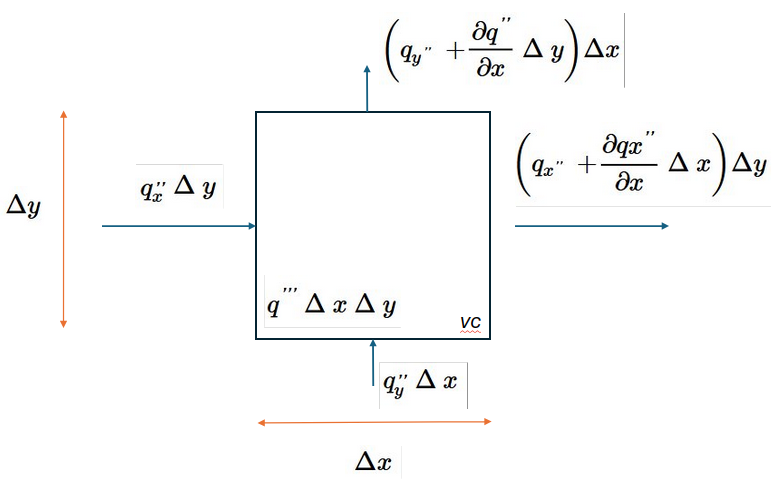
\includegraphics[width=.65\textwidth]{Figures/1_5}
	\caption{Equilíbrio da primeira lei da termodinâmica em volume infinitesimal pelo calor gerado e calor transferido}
\end{figure}

Do anterior, obtêm-se os seguintes termos de acumulação de energia no volume de controle, transferência de energia por fluxo, transferência de calor por condução, calor gerado e fluxo de trabalho, respectivamente
\begin{equation}
	 \Delta x \Delta y  \Delta z \frac{\partial}{\partial t} (\rho e)
\end{equation}

\begin{equation}
	 - (\Delta x \Delta y \Delta z) 
	\left[ \frac{\partial}{\partial x} (\rho u e) + \frac{\partial}{\partial y} (\rho v e) \frac{\partial}{\partial z} (\rho w e)\right]
\end{equation}

\begin{equation}
	 - (\Delta x \Delta y \Delta z) 
	\left( \frac{\partial q_x''}{\partial x} + \frac{\partial q_y''}{\partial y} + \frac{\partial q_z''}{\partial z} \right)
\end{equation}

\begin{equation}
	(\Delta x \Delta y \Delta z) q'''
\end{equation}

\begin{equation}
	\begin{aligned}
	(\Delta x \Delta y \Delta z) \left( \sigma_x \frac{\partial u}{\partial x} - \tau_{xy} \frac{\partial u}{\partial y} + \sigma_y \frac{\partial v}{\partial y} - \tau_{yx} \frac{\partial v}{\partial x} + \sigma_z \frac{\partial w}{\partial z} - \tau_{zx} \frac{\partial w}{\partial x} \right ) + (\Delta x \Delta y \Delta z) \\
	\left( u \frac{\partial \sigma_x}{\partial x} - u \frac{\partial \tau_{xy}}{\partial y} + v \frac{\partial \sigma_y}{\partial y} - v \frac{\partial \tau_{yx}}{\partial x} + w \frac{\partial \sigma_z}{\partial z} - w \frac{\partial \tau_{xz}}{\partial z} \right)
\end{aligned}
\end{equation}

Onde $e$ é a energia específica, $q''$ o fluxo de calor na direção descrita e $q'''$ a dissipação do calor interno gerado. Usando esses termos dentro da expressão de conservação de energia obtemos

\begin{equation}
	\begin{aligned}
		\rho \frac{ De}{Dt} + e(\frac{D}{D t} \rho +  \bigtriangledown (\rho V)) = -\bigtriangledown q'' + q''' - P\bigtriangledown V + \mu \phi
	\end{aligned}
\end{equation}

A função de dissipação viscosa sendo

\begin{equation}
	\begin{aligned}
		\phi = 2[(\frac{\partial u}{\partial x})^{2} + (\frac{\partial v}{\partial y})^{2} + (\frac{\partial w}{\partial z})^{2}] + (\frac{\partial u}{\partial y} + \frac{\partial v}{\partial x} + \frac{\partial w}{\partial z})^{2}
	\end{aligned}
\end{equation}

\textbf{Regime permanente:} 

Para conservação da massa
\begin{equation}
	\begin{aligned}
		  \bigtriangledown (\rho V)= 0 
	\end{aligned}
\end{equation}

De momento:
\begin{equation}
	\begin{aligned}
		\frac{\partial}{\partial x} (\rho u u) + \frac{\partial}{\partial y} (\rho v u) + \frac{\partial}{\partial z} (\rho w u) = \\
		- \frac{\partial p}{\partial x} + \frac{\partial}{\partial x} \left( 2 \mu \frac{\partial u}{\partial x} + \lambda \nabla \cdot \mathbf{V} \right) +
		\frac{\partial}{\partial y} \left( \mu \left( \frac{\partial u}{\partial y} + \frac{\partial v}{\partial x} \right) \right) +
		\frac{\partial}{\partial z} \left( \mu \left( \frac{\partial u}{\partial z} + \frac{\partial w}{\partial x} \right) \right) + g_x
	\end{aligned}
\end{equation}

\begin{equation}
	\begin{aligned}
		\frac{\partial}{\partial x} (\rho u v) + \frac{\partial}{\partial y} (\rho v v) + \frac{\partial}{\partial z} (\rho w v) = \\
		- \frac{\partial p}{\partial y} + \frac{\partial}{\partial x} \left( \mu \left( \frac{\partial v}{\partial x} + \frac{\partial u}{\partial y} \right) \right) +
		\frac{\partial}{\partial y} \left( 2 \mu \frac{\partial v}{\partial y} + \lambda \nabla \cdot \mathbf{V} \right) +
		\frac{\partial}{\partial z} \left( \mu \left( \frac{\partial v}{\partial z} + \frac{\partial w}{\partial y} \right) \right) +  g_y
	\end{aligned}
\end{equation}

\begin{equation}
	\begin{aligned}
		 \frac{\partial}{\partial x} (\rho u w) + \frac{\partial}{\partial y} (\rho v w) + \frac{\partial}{\partial z} (\rho w w) = \\
		- \frac{\partial p}{\partial z} + \frac{\partial}{\partial x} \left( \mu \left( \frac{\partial w}{\partial x} + \frac{\partial u}{\partial z} \right) \right) +
		\frac{\partial}{\partial y} \left( \mu \left( \frac{\partial w}{\partial y} + \frac{\partial v}{\partial z} \right) \right) +
		\frac{\partial}{\partial z} \left( 2 \mu \frac{\partial w}{\partial z} + \lambda \nabla \cdot \mathbf{V} \right) +  g_z
	\end{aligned}
\end{equation}

E de energia:
\begin{equation}
	\begin{aligned}
		 e( \rho +  \bigtriangledown (\rho V)) = -\bigtriangledown q'' + q''' - P\bigtriangledown V + \mu \phi
	\end{aligned}
\end{equation}

\textbf{Laminar:}
Para fluxos laminares, os efeitos advectivos são negligenciados em números de Reynolds baixos. Portanto, há maiores efeitos dos fenômenos viscosos

\begin{equation}
	\begin{aligned}
		\frac{\partial}{\partial t} (\rho u)=
		- \frac{\partial p}{\partial x} + \frac{\partial}{\partial x} \left( 2 \mu \frac{\partial u}{\partial x} + \lambda \nabla \cdot \mathbf{V} \right) +
		\frac{\partial}{\partial y} \left( \mu \left( \frac{\partial u}{\partial y} + \frac{\partial v}{\partial x} \right) \right) +
		\frac{\partial}{\partial z} \left( \mu \left( \frac{\partial u}{\partial z} + \frac{\partial w}{\partial x} \right) \right) + g_x
	\end{aligned}
\end{equation}


\begin{equation}
	\begin{aligned}
		\frac{\partial}{\partial t} (\rho v)  = 
		- \frac{\partial p}{\partial y} + \frac{\partial}{\partial x} \left( \mu \left( \frac{\partial v}{\partial x} + \frac{\partial u}{\partial y} \right) \right) +
		\frac{\partial}{\partial y} \left( 2 \mu \frac{\partial v}{\partial y} + \lambda \nabla \cdot \mathbf{V} \right) +
		\frac{\partial}{\partial z} \left( \mu \left( \frac{\partial v}{\partial z} + \frac{\partial w}{\partial y} \right) \right) +  g_y
	\end{aligned}
\end{equation}

\begin{equation}
	\begin{aligned}
		\frac{\partial}{\partial t} (\rho w) =
		- \frac{\partial p}{\partial z} + \frac{\partial}{\partial x} \left( \mu \left( \frac{\partial w}{\partial x} + \frac{\partial u}{\partial z} \right) \right) +
		\frac{\partial}{\partial y} \left( \mu \left( \frac{\partial w}{\partial y} + \frac{\partial v}{\partial z} \right) \right) +
		\frac{\partial}{\partial z} \left( 2 \mu \frac{\partial w}{\partial z} + \lambda \nabla \cdot \mathbf{V} \right) +  g_z
	\end{aligned}
\end{equation}
 
\textbf{Incompressivel:}

Para conservação da massa
\begin{equation}
	\begin{aligned}
		\bigtriangledown (\rho V)= 0 
	\end{aligned}
\end{equation}

Para conservação de momento:

\begin{equation}
	\begin{aligned}
		 \rho(\frac{\partial}{\partial x} ( u u) + \frac{\partial}{\partial y} (v u) + \frac{\partial}{\partial z} (w u) )= \\
		- \frac{\partial p}{\partial x} + \frac{\partial}{\partial x} \left( 2 \mu \frac{\partial u}{\partial x} + \lambda \nabla \cdot \mathbf{V} \right) +
		\frac{\partial}{\partial y} \left( \mu \left( \frac{\partial u}{\partial y} + \frac{\partial v}{\partial x} \right) \right) +
		\frac{\partial}{\partial z} \left( \mu \left( \frac{\partial u}{\partial z} + \frac{\partial w}{\partial x} \right) \right) + g_x
	\end{aligned}
\end{equation}

E para $y$ e $z$

\begin{equation}
	\begin{aligned}
		 \rho(\frac{\partial}{\partial x} ( u v) + \frac{\partial}{\partial y} ( v v) + \frac{\partial}{\partial z} ( w v)) = \\
		- \frac{\partial p}{\partial y} + \frac{\partial}{\partial x} \left( \mu \left( \frac{\partial v}{\partial x} + \frac{\partial u}{\partial y} \right) \right) +
		\frac{\partial}{\partial y} \left( 2 \mu \frac{\partial v}{\partial y} + \lambda \nabla \cdot \mathbf{V} \right) +
		\frac{\partial}{\partial z} \left( \mu \left( \frac{\partial v}{\partial z} + \frac{\partial w}{\partial y} \right) \right) +  g_y
	\end{aligned}
\end{equation}

\begin{equation}
	\begin{aligned}
		\rho(\frac{\partial}{\partial x} ( u w) + \frac{\partial}{\partial y} ( v w) + \frac{\partial}{\partial z} ( w w)) = \\
		- \frac{\partial p}{\partial z} + \frac{\partial}{\partial x} \left( \mu \left( \frac{\partial w}{\partial x} + \frac{\partial u}{\partial z} \right) \right) +
		\frac{\partial}{\partial y} \left( \mu \left( \frac{\partial w}{\partial y} + \frac{\partial v}{\partial z} \right) \right) +
		\frac{\partial}{\partial z} \left( 2 \mu \frac{\partial w}{\partial z} + \lambda \nabla \cdot \mathbf{V} \right) +  g_z
	\end{aligned}
\end{equation}
E para energia:
\begin{equation}
	\begin{aligned}
		\rho \frac{ De}{Dt} + e\rho(  \bigtriangledown (\rho V) = -\bigtriangledown q'' + q''' - P\bigtriangledown V + \mu \phi
	\end{aligned}
\end{equation}

\textbf{Propiedades constantes:}

Para conservação da massa
\begin{equation}
	\begin{aligned}
		\bigtriangledown (\rho V)= 0 
	\end{aligned}
\end{equation}

Para conservacao de momento:
\begin{equation}
	\begin{aligned}
		\rho(\frac{\partial}{\partial x} ( u u) + \frac{\partial}{\partial y} (v u) + \frac{\partial}{\partial z} (w u) )= \\
		- \frac{\partial p}{\partial x} +2 \mu \frac{\partial}{\partial x} \left(  \frac{\partial u}{\partial x} + \lambda \nabla \cdot \mathbf{V} \right) + \mu
		\frac{\partial}{\partial y} \left(  \left( \frac{\partial u}{\partial y} + \frac{\partial v}{\partial x} \right) \right) + \mu
		\frac{\partial}{\partial z} \left(  \left( \frac{\partial u}{\partial z} + \frac{\partial w}{\partial x} \right) \right) + g_x
	\end{aligned}
\end{equation}

E para $y$ e $z$

\begin{equation}
	\begin{aligned}
		\rho(\frac{\partial}{\partial x} ( u v) + \frac{\partial}{\partial y} ( v v) + \frac{\partial}{\partial z} ( w v)) = \\
		- \frac{\partial p}{\partial y} + \mu \frac{\partial}{\partial x} \left(  \left( \frac{\partial v}{\partial x} + \frac{\partial u}{\partial y} \right) \right) + 2 \mu
		\frac{\partial}{\partial y} \left(  \frac{\partial v}{\partial y} + \lambda \nabla \cdot \mathbf{V} \right) +\mu
		\frac{\partial}{\partial z} \left(  \left( \frac{\partial v}{\partial z} + \frac{\partial w}{\partial y} \right) \right) +  g_y
	\end{aligned}
\end{equation}

\begin{equation}
	\begin{aligned}
		\rho(\frac{\partial}{\partial x} ( u w) + \frac{\partial}{\partial y} ( v w) + \frac{\partial}{\partial z} ( w w)) = \\
		- \frac{\partial p}{\partial z} + \mu \frac{\partial}{\partial x} \left(  \left( \frac{\partial w}{\partial x} + \frac{\partial u}{\partial z} \right) \right) + \mu
		\frac{\partial}{\partial y} \left(  \left( \frac{\partial w}{\partial y} + \frac{\partial v}{\partial z} \right) \right) + 2 \mu
		\frac{\partial}{\partial z} \left(  \frac{\partial w}{\partial z} + \lambda \nabla \cdot \mathbf{V} \right) +  g_z
	\end{aligned}
\end{equation}
E para energia, na lei de Fourier fican $Cp$ e $k$ constantes

\textbf{Dissipação viscosa desprezível:}
Na ecuação de energia elimina-se $\phi$:

\begin{equation}
	\begin{aligned}
		\rho \frac{ De}{Dt} + e(\frac{D}{D t} \rho +  \bigtriangledown (\rho V)) = -\bigtriangledown q'' + q''' - P\bigtriangledown V 
	\end{aligned}
\end{equation}


\begin{thebibliography}{999}
	
	\bibitem{abejan}
	Adrian Bejan,
	Convection Heat Transfer.
	Durham, North Carolina,
	3rd Edition,
	2004.
	
	\bibitem{abejan}
	Clovis Maliska,
	Transferência de calor e mecânica dos fluidos computacional.
	UFSC,Brasil,
	2nd Edition,
	2004.
	
\end{thebibliography}
\end{document}





